\documentclass[11pt]{article}
\usepackage{acl}
\usepackage{times}
\usepackage{latexsym}
\usepackage{graphicx}
\usepackage{booktabs}
\usepackage{amsmath}
\usepackage{multirow}
\usepackage{xcolor}
\usepackage{url}
\usepackage{tabularx}
\usepackage[T1]{fontenc}
\usepackage[utf8]{inputenc}

\title{Do Structured Data Comprehension Skills Transfer Across Representation Types?\\A Systematic Study with Frontier LLMs}

\author{Farseen Shaikh \\
  Independent Researcher \\
  \texttt{farseenshaikh20@gmail.com}}

\begin{document}
\maketitle

% ============================================================
\begin{abstract}
Large language models (LLMs) are increasingly evaluated on structured data tasks---table question answering, chart comprehension, graph reasoning, and time series analysis---yet these benchmarks operate in isolation. We ask: \emph{does competence in one structured data format predict competence in another when the underlying data and questions are identical?}

We construct a controlled benchmark of 1,724 programmatically generated questions over 250 sub-tables drawn from 10 datasets spanning 7 domains. Each sub-table is rendered in five formats: Markdown table, chart image, chart text-description, entity-relationship graph, and unlabeled time series. We evaluate six frontier March 2026 LLMs and measure cross-format transfer via tetrachoric correlation on binary (correct/incorrect) outcomes.

Our key findings: (1)~structured data comprehension skills \textbf{transfer strongly} across text-based formats, with mean tetrachoric $r{=}0.87$ between table, graph, and time series representations across all six models ($r{=}0.84$ for the three mid-range models, confirming the result is not an artifact of near-ceiling accuracy); (2)~chart text-descriptions show consistently lower transfer ($r{=}0.65$) despite being length-matched to tables; (3)~chart image comprehension is largely \textbf{siloed}, with a 20--50\% accuracy gap compared to equivalent text descriptions; and (4)~enabling chain-of-thought reasoning improves text-format accuracy by 24--38\% for DeepSeek V3.2 but only 0--0.5\% for Gemini 3.1 Pro (with a $+2$\% chart-image gain), suggesting reasoning benefits may vary substantially across models, though this observation is based on two models and requires further validation. On hard questions (multi-hop and conditional aggregation), transfer is at least as strong as on basic questions ($r{=}0.85$ vs $r{=}0.81$ for the table-graph-timeseries cluster).
\end{abstract}

% ============================================================
\section{Introduction}

The ability of large language models to understand structured data has been evaluated through an expanding ecosystem of benchmarks: WikiTableQuestions \cite{pasupat2015compositional} and TabFact \cite{chen2020tabfact} for tables, ChartQA \cite{masry2022chartqa} and ChartQAPro \cite{chartqapro2025} for charts, GraphOmni \cite{graphomni2026} for graphs, and TSAQA \cite{tsaqa2026} for time series. Each benchmark evaluates models on a single representation type in isolation.

This siloed evaluation leaves a fundamental question unanswered: \emph{are structured data comprehension skills format-specific, or do they reflect a general capability that transfers across representations?} By ``transfer,'' we mean cross-format consistency: does a model that answers a question correctly in one format also answer it correctly in another, beyond what chance agreement would predict? If a model excels at extracting values from a Markdown table, can we predict it will also succeed when the same data is presented as a graph or time series?

Understanding cross-format transfer has practical implications. If skills are siloed, developers must test models on each target format independently. If skills transfer, a single benchmark may suffice to predict broader structured data competence. Furthermore, format-specific weaknesses may reveal architectural limitations amenable to targeted improvement.

We extend prior controlled-content methodology---most notably \citet{zhang2026samecontent}, who isolate representation effects within table-only variations---to span five fundamentally different representation types (table, chart image, chart text, graph-like serialization, time series) under identical content and programmatic ground truth. Our contributions are:

\begin{enumerate}
    \item A controlled benchmark of 1,724 questions where \textbf{identical data and questions} are presented in five formats, enabling direct comparison unconfounded by content variation.
    \item Cross-format transfer measurements via \textbf{tetrachoric correlation} on six frontier March 2026 models, finding strong transfer ($r{>}0.85$) among text-based formats but moderate-to-weak transfer involving chart descriptions ($r{\approx}0.65$).
    \item Evidence that \textbf{chart image comprehension is siloed}: vision-based chart reading lags text equivalents by 20--50\%, even when the underlying data is identical.
    \item A \textbf{reasoning ablation} showing chain-of-thought benefits are model-dependent: DeepSeek V3.2 gains 30+ percentage points while Gemini 3.1 Pro gains under 1\%.
\end{enumerate}

% ============================================================
\section{Related Work}

\paragraph{Table QA.} Table question answering has advanced rapidly. Recent multi-agent approaches such as Orchestra \cite{orchestra2026} approach GPT-4's prior 75.3\% EM benchmark on WikiTableQuestions \cite{pasupat2015compositional} using smaller open-weight models, and MCTS-based agentic frameworks such as TabTracer \cite{tabtracer2026} report up to 6.7\% accuracy improvements over prior state-of-the-art on TabFact \cite{chen2020tabfact} and WikiTQ. MMTU \cite{mmtu2025} extends evaluation to a multi-task table understanding suite covering 25 task types over diverse domains.

\paragraph{Chart Comprehension.} ChartQA \cite{masry2022chartqa} established chart QA as a benchmark; frontier vision-language models have approached saturation, with Claude Sonnet 3.5 scoring 90.5\% \cite{chartqapro2025}. ChartQAPro \cite{chartqapro2025} introduced harder questions where the current best (Claude 3.5 with CoT) reaches only 55.81\%. CharXiv \cite{charxiv2024} and ChartMuseum \cite{chartmuseum2025} further challenge models on real-world scientific charts. \citet{infochartqa2025} pair infographic and plain charts sharing identical underlying data, finding substantial accuracy drops on the infographic variant.

\paragraph{Graph Reasoning.} GraphOmni \cite{graphomni2026} demonstrated that serialization format dramatically affects LLM performance on graph-theoretic tasks across 7 graph types and 7 serialization formats, while GraCoRe \cite{gracore2025} reports persistent capability gaps on complex graph reasoning across 19 tasks.

\paragraph{Time Series.} \citet{tsaqa2026} introduced a unified time-series QA benchmark spanning six tasks; their best accuracy on the puzzling format is 67.68\% with a fine-tuned LLaMA-3.1-8B, indicating substantial room for improvement. \citet{mmtsbench2026} report that general-purpose LLMs with chain-of-thought reasoning outperform specialized time-series-adapted LLMs. \citet{hearts2026} show that LLM performance on health time-series tasks declines with increasing temporal complexity.

\paragraph{Cross-Format Studies.} Most closely related to our work, \citet{zhang2026samecontent} present a controlled study isolating the role of table representation by holding content constant. Their scope is table-only (structured vs.\ semi-structured tables). \citet{liu2025formatprior} quantify format-as-prior bias in LLMs across heterogeneous data, focusing on bias rather than transfer. \citet{ho2025formatmatters} characterize the robustness of multimodal LLMs in reviewing evidence from tables and charts. \citet{bhandari2026tabular} show that semantically equivalent table serializations produce substantially different retrieval embeddings, addressing format sensitivity at the encoder level. \citet{epoch2026}'s benchmark-stitching analysis and \citet{ilic2023gfactor}'s factor-analytic study examine general capability factors across LLM benchmarks but not within structured data specifically.

Additionally, ToRR \cite{torr2026} studies multi-format table robustness across varied serializations, finding that evaluating across formats is essential for reliable assessment. WikiMixQA \cite{wikimixqa2025} evaluates cross-modal reasoning over tables and charts from the same Wikipedia pages. DataCross \cite{datacross2026} spans SQL/CSV and visual document types for cross-modal benchmarking. However, all of these either remain within a single modality (tables) or test different questions across formats.

We extend the controlled-content methodology of \citet{zhang2026samecontent}---who isolate representation effects within table-only variations---to span \textbf{five fundamentally different representation types} (table, chart image, chart text, graph-like serialization, time series) while keeping data and questions identical. This combination of strict same-content control, question-level paired measurement via tetrachoric correlation, and cross-modality scope is not present in any prior work to our knowledge.

% ============================================================
\section{Methodology}

\subsection{Data Construction}

We extract 250 sub-tables from 10 publicly available datasets spanning 7 domains: governance/economics, transportation, energy (2 datasets), agriculture (2 datasets), air quality (2 datasets), transit, and finance. Sub-tables are sampled at three complexity tiers: small (5$\times$3, $n{=}$80), medium (10$\times$5, $n{=}$100), and large (20$\times$8, $n{=}$70).

\subsection{Five Representation Formats}

Each sub-table is rendered in five formats:

\begin{description}
    \item[Format A (Table):] Standard Markdown table with headers and aligned columns.
    \item[Format B (Chart Image):] Matplotlib-generated PNG chart (bar, line, or scatter, selected by data properties).
    \item[Format B$'$ (Chart Text):] Natural language description of the chart, length-matched to Format A within $\pm$20\% tokens (100\% compliance achieved using cl100k\_base tokenizer).
    \item[Format C (Graph):] Entity-relationship text representation with node attributes and top-$K$ edges by metric cosine similarity, where $K{=}\max(3, \lfloor N/2 \rfloor)$ for $N$ entities. Note: this is a constructed serialization of tabular data into graph-like text, not a natural graph structure. We use ``graph'' as shorthand throughout but acknowledge this distinction.
    \item[Format D (Time Series):] Unlabeled numerical arrays with positional headers, forcing index-based reasoning.
\end{description}

Format B$'$ serves as a \textbf{modality control}: it contains the same information as Format B (chart) but in text, isolating the effect of visual processing from chart comprehension.

\paragraph{Format examples.} To illustrate, consider a sub-table of European energy data with columns \texttt{Entity}, \texttt{Coal\_GWh}, \texttt{Solar\_GWh}, and \texttt{Wind\_GWh} for five countries. Format~A presents this as a standard pipe-delimited Markdown table. Format~B renders it as a grouped bar chart PNG. Format~B$'$ describes the same chart in prose: ``Bar chart: `OPSD Electricity --- Energy'. Coal\_GWh: Denmark=920.8, Germany=3542.1, \ldots'', explicitly listing each data point. Format~C represents entities as graph nodes with attributes (e.g., ``Denmark: \{Coal\_GWh=920.8, Solar\_GWh=3001.0, Wind\_GWh=503.5\}'') and edges between entities with high metric cosine similarity. Format~D strips all labels, presenting only ordered numerical arrays: ``The following 5 values represent Coal\_GWh for each Entity (Denmark, Germany, \ldots), listed in order: [920.8, 3542.1, \ldots]''.

This design ensures that every format contains sufficient information to answer all seven question types, while varying the \emph{structure} through which the information is accessed. The key design constraint is that no format omits data---differences in accuracy are attributable to format difficulty, not information asymmetry.

\subsection{Question Generation}

We generate seven question types with deterministic ground truth computed via \texttt{pandas}:

\begin{itemize}
    \item \textbf{Q1 (Lookup):} Direct value retrieval.
    \item \textbf{Q2 (Comparison):} Binary comparison between entities.
    \item \textbf{Q3 (Aggregation):} Mean computation across entities.
    \item \textbf{Q4 (Trend):} Directional change (increase/decrease).
    \item \textbf{Q5 (Extremum):} Maximum/minimum identification.
    \item \textbf{Q6 (Multi-hop):} Two-step reasoning (find max of metric A, report metric B). Tie-breaking: exclude if top-2 gap $<$5\%.
    \item \textbf{Q7 (Conditional Aggregation):} Filter-then-aggregate. Threshold selected for 30--70\% row pass rate.
\end{itemize}

This yields 1,724 questions (250 sub-tables $\times$ 7 types, minus 26 Q6 exclusions from tie-breaking). All scoring is deterministic: exact match for categorical answers, numerical tolerance ($\pm$2\% for lookup/multi-hop, $\pm$5\% for aggregation).

\subsection{Models}

We evaluate six frontier LLMs available in March 2026 (Table~\ref{tab:models}). Three support vision input for Format B evaluation; all six are evaluated on the four text formats.

\begin{table}[t]
\centering
\small
\begin{tabular}{lcc}
\toprule
\textbf{Model} & \textbf{Vision} & \textbf{Reasoning} \\
\midrule
DeepSeek V3.2 & No & Enabled \\
MiniMax M2.5 & No & Default on \\
Kimi K2.5 & Yes & Default on \\
GLM-5 & No & Default on \\
Qwen 3.5 Plus & Yes & Default on \\
Gemini 3.1 Pro & Yes & Thinking on \\
\bottomrule
\end{tabular}
\caption{Models evaluated. Reasoning indicates whether chain-of-thought/extended thinking was active during evaluation. All models use their default or recommended reasoning configuration.}
\label{tab:models}
\end{table}

\subsection{Metrics}

Our primary metric is \textbf{tetrachoric correlation} \cite{divgi1979calculation}, computed via the \texttt{ordinalcorr} library (v0.6.1). Tetrachoric correlation estimates the latent Pearson correlation between two continuous variables from their dichotomized (binary) observations, making it appropriate for our correct/incorrect scoring. We report phi coefficients as a secondary metric and bootstrap 95\% confidence intervals (2,000 resamples). For interpretation: $r{=}0.85$ implies that approximately 72\% of the variance in one format's performance is explained by another format's performance ($r^2{=}0.72$), indicating strong predictability across formats.

\subsection{Token Counts}

Median token counts (cl100k\_base) per format: Table 276, Chart Text 270, Graph 520, Time Series 380. The Chart Text/Table ratio is 1.04 (median), confirming successful length matching. Graph representations are approximately 2$\times$ longer due to edge descriptions; we note this as a potential confound.

% ============================================================
\section{Results}

\subsection{Overall Accuracy}

Table~\ref{tab:accuracy} presents per-format accuracy across all six models. Several patterns emerge consistently:

\begin{table*}[t]
\centering
\small
\begin{tabular}{lccccc}
\toprule
\textbf{Model} & \textbf{Table} & \textbf{Chart Text} & \textbf{Graph} & \textbf{Time Series} & \textbf{Chart Image} \\
\midrule
DeepSeek V3.2 & 97.3 {\scriptsize[97--98]} & 88.7 {\scriptsize[87--90]} & 97.9 {\scriptsize[97--98]} & 96.9 {\scriptsize[96--98]} & --- \\
MiniMax M2.5 & 95.8 {\scriptsize[95--97]} & 87.2 {\scriptsize[86--89]} & 96.3 {\scriptsize[95--97]} & 94.8 {\scriptsize[94--96]} & --- \\
Kimi K2.5 & 89.1 {\scriptsize[88--90]} & 81.6 {\scriptsize[80--83]} & 88.8 {\scriptsize[87--90]} & 87.8 {\scriptsize[86--89]} & 31.9 {\scriptsize[30--34]} \\
GLM-5 & 88.8 {\scriptsize[87--90]} & 81.3 {\scriptsize[79--83]} & 88.9 {\scriptsize[87--90]} & 88.8 {\scriptsize[87--90]} & --- \\
Qwen 3.5 Plus & 99.2 {\scriptsize[99--100]} & 90.1 {\scriptsize[89--91]} & 99.2 {\scriptsize[99--100]} & 99.4 {\scriptsize[99--100]} & 58.9 {\scriptsize[57--61]} \\
Gemini 3.1 Pro & 99.4 {\scriptsize[99--100]} & 90.1 {\scriptsize[89--91]} & 99.2 {\scriptsize[99--100]} & 99.3 {\scriptsize[99--100]} & 70.6 {\scriptsize[68--73]} \\
\bottomrule
\end{tabular}
\caption{Accuracy (\%) by format with 95\% Wilson confidence intervals. Chart image evaluation conducted on the three vision-capable models; the remaining three models were evaluated on Format B$'$ (chart text-description). Dashes indicate non-vision models.}
\label{tab:accuracy}
\end{table*}

Three patterns emerge consistently. First, accuracy on the table, graph-like, and time-series formats is within 1--3 percentage points for every model, suggesting a shared underlying comprehension skill across these three text-based representations. Second, despite length-matching to $\pm$20\% tokens, chart-text descriptions consistently lag tables by 7--9\% across all six models, indicating a systematic information-loss penalty for prose-formatted structured data. Third, chart images are the clear outlier: among the three vision-capable models, chart-image accuracy ranges from 31.9\% (Kimi K2.5) to 70.6\% (Gemini 3.1 Pro)---dramatically lower than the 81--99\% achieved on text formats with identical data.

\subsection{Cross-Format Transfer}

Figure~\ref{fig:heatmap} presents the averaged tetrachoric correlation matrix across all six models on the four text formats.

\begin{figure}[t]
    \centering
    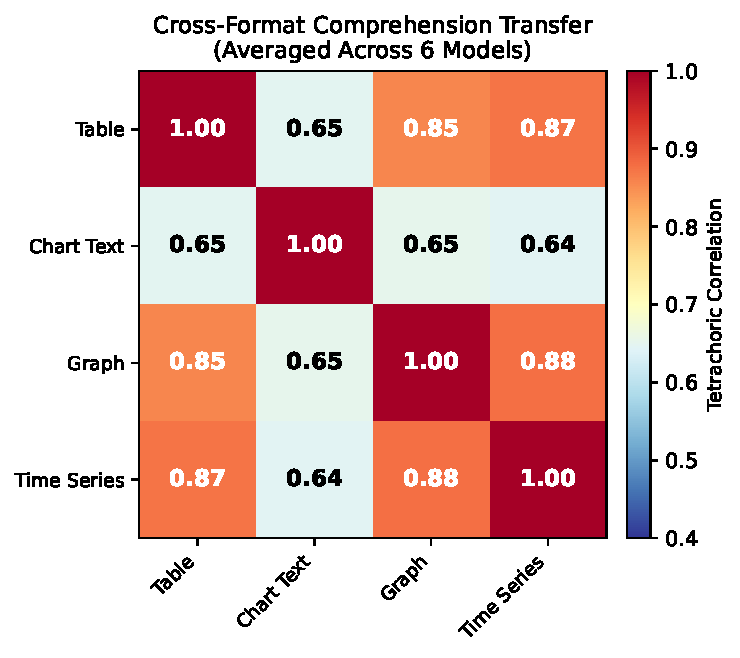
\includegraphics[width=\columnwidth]{fig1_correlation_heatmap.pdf}
    \caption{Tetrachoric correlation of question-level accuracy across four text-based formats, averaged over six models. Table, Graph, and Time Series show strong mutual transfer ($r{>}0.85$), while Chart Text shows moderate transfer ($r{\approx}0.65$).}
    \label{fig:heatmap}
\end{figure}

The correlation structure reveals two clusters:
\begin{itemize}
    \item \textbf{High transfer ($r{=}0.86$--0.88):} Table~$\leftrightarrow$~Graph, Table~$\leftrightarrow$~Time Series, Graph~$\leftrightarrow$~Time Series. Models that answer a question correctly in one of these formats overwhelmingly answer it correctly in the others.
    \item \textbf{Moderate transfer ($r{=}0.64$--0.65):} Chart Text with all other formats. The narrative description format introduces systematic difficulty that is partially orthogonal to the skills tested by other formats.
\end{itemize}

\paragraph{Ceiling effect robustness check.} Three models (Qwen, Gemini, DeepSeek) achieve $\geq$95\% mean text-format accuracy, raising the concern that high tetrachoric correlations are artifacts of near-ceiling accuracy rather than genuine transfer. We address this by splitting models into a \textbf{ceiling group} ($\geq$95\% mean accuracy; $n{=}3$) and a \textbf{mid-range group} ($<$95\%; Kimi, GLM-5, MiniMax; $n{=}3$). The mid-range group shows averaged tetrachoric $r{=}0.84$ for table-graph-timeseries pairs and $r{=}0.67$ for chart text pairs---closely matching the overall all-six-model values of $r{=}0.87$ and $r{=}0.65$, respectively. The ceiling group shows slightly higher values ($r{=}0.90$ and $r{=}0.63$) as expected, but the difference between the two groups is modest. We conclude that the strong-transfer finding is \textbf{not} an artifact of ceiling effects. Within the ceiling group, however, per-model correlations vary substantially (DeepSeek $r{=}0.73$ vs Qwen $r{=}0.99$), reflecting tetrachoric correlation's known instability at extreme base rates; the mid-range estimate ($r{=}0.84$) should therefore be interpreted as the more conservative point estimate.

\subsection{Question Type Analysis}

Table~\ref{tab:qtype} shows accuracy by question type, averaged across all models and text formats.

\begin{table}[t]
\centering
\small
\begin{tabular}{lcc}
\toprule
\textbf{Question Type} & \textbf{Avg Acc.} & \textbf{Range} \\
\midrule
Q4 Trend & 97.6\% & 92--100\% \\
Q1 Lookup & 92.5\% & 83--98\% \\
Q2 Comparison & 94.3\% & 89--97\% \\
Q5 Extremum & 91.3\% & 86--96\% \\
Q6 Multi-hop & 91.7\% & 80--98\% \\
Q3 Aggregation & 85.8\% & 71--94\% \\
Q7 Cond. Aggregation & 68.0\% & 30--88\% \\
\bottomrule
\end{tabular}
\caption{Accuracy by question type, averaged across 6 models over each model's evaluated formats (4 text formats for non-vision models; 4 text + 1 chart-image for vision models). Q7 conditional aggregation provides the strongest discrimination.}
\label{tab:qtype}
\end{table}

Q7 (conditional aggregation) is the most discriminating question type, with accuracy ranging from 29.7\% (Kimi K2.5) to 87.8\% (Gemini 3.1 Pro). This two-step filter-then-aggregate operation tests both data extraction and arithmetic skills simultaneously.

\paragraph{Interaction between question type and format.} The format effect is not uniform across question types. For simple operations (Q1 lookup, Q4 trend), all text formats achieve $>$90\% accuracy regardless of model, and the cross-format correlation is near-perfect ($r{>}0.95$). The gap emerges on computational questions: Q3 (aggregation) and Q7 (conditional aggregation) show the largest format-dependent variance. On Q7 specifically, Chart Text accuracy is approximately 10 percentage points lower than Table accuracy on average, compared to approximately 7 points lower for Q1; on Q3 (aggregation) the format-dependent gap reaches approximately 17 points. This suggests that the prose format particularly hinders multi-step numerical reasoning, likely because intermediate values must be extracted from flowing text rather than directly indexed from a structured representation.

\paragraph{Per-model variation.} While the format ranking (Table~$\geq$~Graph~$\geq$~Time Series~$>$~Chart Text~$\gg$~Chart Image) is consistent across models, the \emph{magnitude} of the gaps varies substantially. Kimi K2.5 and GLM-5 show 8--9\% gaps between Table and Chart Text, similar in magnitude to Qwen 3.5 Plus and Gemini 3.1 Pro (9\% gap, but from a higher baseline). Interestingly, the two strongest models (Qwen and Gemini) show nearly identical accuracy profiles across all five formats, despite being trained by different organizations with different architectures. This convergence suggests a common ceiling for structured data comprehension in frontier models.

\subsection{Modality Isolation: Chart Image vs.\ Chart Text}

Format B$'$ (Chart Text) was designed to isolate the effect of visual processing from chart comprehension. Figure~\ref{fig:modality} shows the comparison for the three vision-capable models.

\begin{figure}[t]
    \centering
    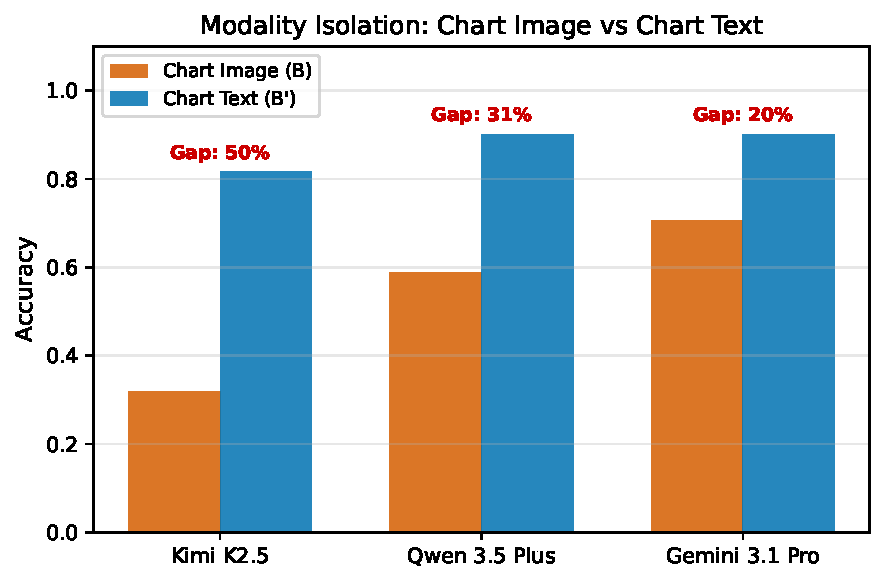
\includegraphics[width=\columnwidth]{fig5_modality_comparison.pdf}
    \caption{Chart Image (B) vs.\ Chart Text (B$'$) accuracy. The gap ranges from 19.6\% (Gemini) to 49.7\% (Kimi), demonstrating that visual chart processing---not chart comprehension per se---is the bottleneck.}
    \label{fig:modality}
\end{figure}

The gaps are substantial: 49.7\% for Kimi K2.5, 31.2\% for Qwen 3.5 Plus, and 19.6\% for Gemini 3.1 Pro. Since the underlying data is identical and the text description contains all information present in the chart, these gaps are attributable entirely to \textbf{visual processing limitations} rather than conceptual difficulty.

\subsection{Error Agreement Analysis}

To further quantify transfer, we examine error \emph{agreement}: when a model answers incorrectly on one format, does it also fail on others? Table~\ref{tab:error_agree} shows the breakdown.

\begin{table}[t]
\centering
\small
\begin{tabular}{lccc}
\toprule
\textbf{Model} & \textbf{All right} & \textbf{All wrong} & \textbf{1-format fail} \\
\midrule
DeepSeek V3.2 & 82.5\% & 0.9\% & 11.3\% \\
MiniMax M2.5 & 82.4\% & 0.8\% & 12.7\% \\
Kimi K2.5 & 75.1\% & 4.6\% & 11.3\% \\
GLM-5 & 74.3\% & 4.4\% & 12.8\% \\
Qwen 3.5 Plus & 89.7\% & 0.5\% & 9.6\% \\
Gemini 3.1 Pro & 89.8\% & 0.5\% & 9.5\% \\
\bottomrule
\end{tabular}
\caption{Error agreement across text formats. ``All right'': correct on all four text formats. ``All wrong'': incorrect on all four. ``1-format fail'': correct on three, wrong on exactly one. The low ``all wrong'' rate (0.3--4.6\%) and high ``all right'' rate (74--90\%) confirm strong cross-format transfer at the question level.}
\label{tab:error_agree}
\end{table}

The results reinforce our correlation findings: 74--90\% of questions are answered identically (correctly) across all four text formats. The ``all wrong'' category is strikingly small (0.3--4.6\%), indicating that truly difficult questions---those that defeat the model regardless of format---are rare. The most informative category is ``1-format fail'' (9.5--12.8\%): these are questions where format \emph{does} matter. Manual inspection reveals these are predominantly Q3 (aggregation) and Q7 (conditional aggregation) questions presented in Chart Text format, consistent with our finding that prose descriptions hinder numerical computation.

\subsection{Domain Effects}

Our 250 sub-tables span seven domains. We find that accuracy varies by domain: agriculture (95.4\%) and energy (94.5\%) are easiest, while transit (90.3\%) and air quality (90.2\%) are hardest, averaged across all models and text formats. Importantly, the \emph{format ranking} (Table~$\geq$~Graph~$\geq$~Time Series~$>$~Chart Text) is preserved within every domain, ruling out domain-specific confounds. The domain variation likely reflects differences in metric naming transparency (e.g., ``GDP\_per\_capita'' is more self-explanatory than ``AQI'') and numerical range distributions.

% ============================================================
\section{Ablations}

\subsection{Reasoning Effect}

We evaluate DeepSeek V3.2 and Gemini 3.1 Pro with and without explicit reasoning (chain-of-thought for DeepSeek, extended thinking for Gemini). Figure~\ref{fig:reasoning} shows the results.

\begin{figure}[t]
    \centering
    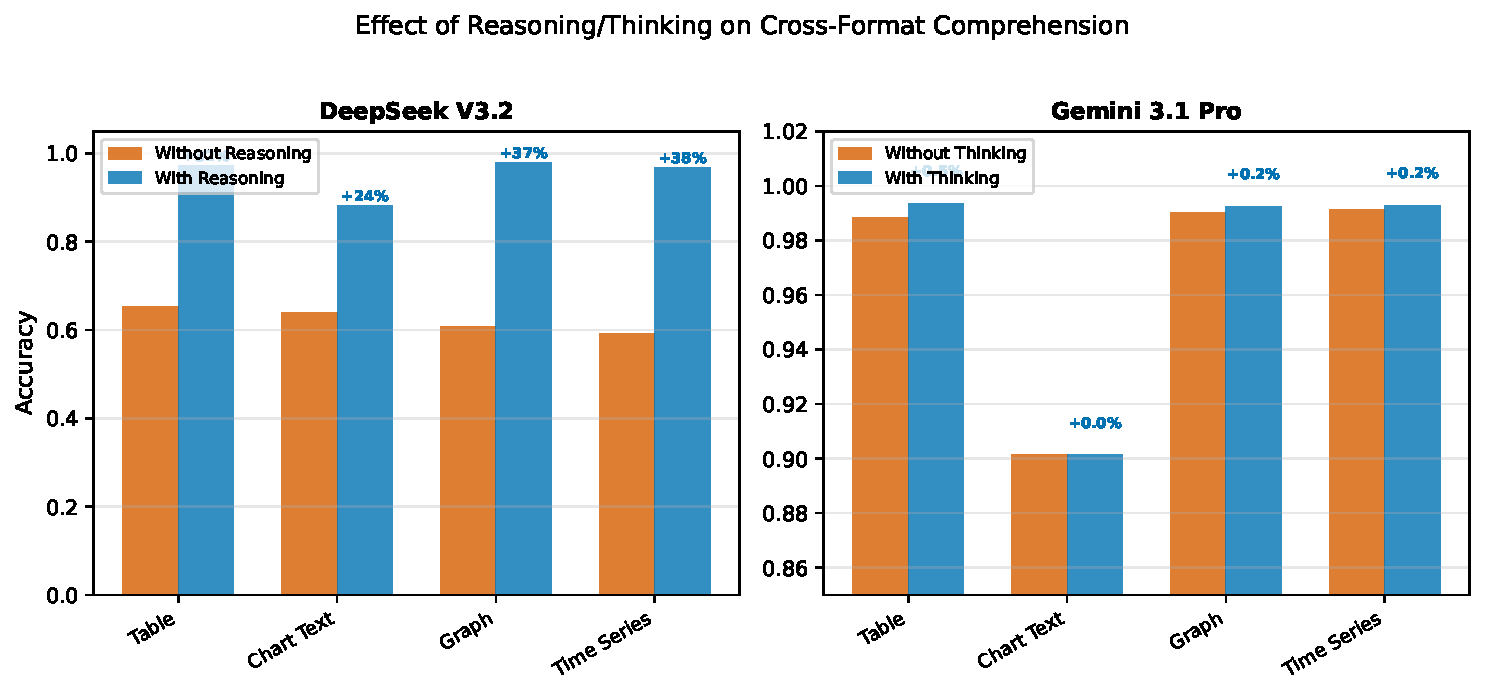
\includegraphics[width=\columnwidth]{fig4_reasoning_ablation.pdf}
    \caption{Effect of reasoning on cross-format comprehension. DeepSeek V3.2 gains 24--38\% on text formats with reasoning enabled; Gemini 3.1 Pro gains $<$1\% on text formats (and $+2$\% on chart images).}
    \label{fig:reasoning}
\end{figure}

DeepSeek V3.2 shows dramatic improvement: Table accuracy jumps from 65.3\% to 97.3\% (+32.0\%), Graph from 60.8\% to 97.9\% (+37.1\%). In contrast, Gemini 3.1 Pro gains at most 0.5\% on any text format (with a $+2.0$\% gain on chart images). This divergence suggests that Gemini's base inference already incorporates sufficient reasoning for structured data tasks, while DeepSeek's chat-oriented architecture requires explicit reasoning to achieve comparable performance.

Crucially, the \emph{relative format ranking} is preserved with and without reasoning for both models. DeepSeek without reasoning shows Table (65.3\%)~$>$~Chart Text (64.0\%)~$>$~Graph (60.8\%)~$>$~Time Series (59.3\%), and with reasoning the ordering becomes Table (97.3\%)~$\approx$~Graph (97.9\%)~$\approx$~Time Series (96.9\%)~$>$~Chart Text (88.7\%). The gap between Chart Text and the other three formats \emph{persists} regardless of reasoning, further confirming that this gap reflects structural information loss rather than insufficient reasoning.

\subsection{Question Difficulty}

We split questions into \textbf{basic} (Q1--Q5, $n{=}$1,250) and \textbf{hard} (Q6--Q7, $n{=}$474). For the table-graph-timeseries cluster, the averaged tetrachoric correlation across all six models is $r{=}0.81$ on basic questions and $r{=}0.85$ on hard questions. Contrary to the intuition that multi-step reasoning would introduce format-dependent difficulty, transfer is at least as strong on hard questions as on basic ones in aggregate, with four of six models (MiniMax, Kimi, GLM-5, Qwen) showing hard $>$ basic correlations; the two exceptions (DeepSeek, Gemini) operate at near-ceiling accuracy where the metric is less stable. This suggests that the cross-format shared capability includes the compositional reasoning required by Q6 (multi-hop) and Q7 (conditional aggregation), not just basic data extraction.

On Q7 specifically---the hardest question type, where Kimi K2.5 achieves only 29.7\% accuracy---transfer correlations remain meaningfully above zero across the mid-range model group, indicating that cross-format consistency persists even on questions where models frequently fail.

\subsection{Complexity Tiers}

Accuracy decreases with sub-table complexity: small (5$\times$3) averages 97.6\%, medium (10$\times$5) averages 92.3\%, and large (20$\times$8) averages 87.7\% across all six models and four text formats. The relative ordering of formats is preserved across tiers, confirming that our findings are not artifacts of data size. The largest tier-by-format interaction is on Chart Text, which degrades more sharply with sub-table size than the other text formats---consistent with the prose format's reliance on sequential scanning rather than direct row-column lookup.

% ============================================================
\section{Discussion}

\paragraph{Skills transfer, modality doesn't.} Our central finding is that structured data comprehension skills \textbf{do transfer} across text-based representation types. A model's ability to look up, compare, aggregate, and reason over data in a Markdown table strongly predicts its ability to do the same when that data is presented as a graph or time series ($r{>}0.85$). This suggests that format-specific benchmarks may be measuring a common underlying capability---at least within text modality. This finding is consistent with the format sensitivity observed by \citet{zhang2026samecontent} within table-only variations and extends it to fundamentally different structured representations, while aligning with the unidimensional capability factor reported by \citet{epoch2026}'s benchmark-stitching analysis and by \citet{ilic2023gfactor}.

However, chart image comprehension is \textbf{siloed}: the correlation between chart image accuracy and text format accuracy is substantially weaker, and the B vs.\ B$'$ comparison confirms that visual processing---not conceptual understanding---is the bottleneck.

\paragraph{Chart Text: the information loss format.} Despite careful length matching, Chart Text consistently underperforms Table by 7--9\%. We hypothesize that the conversion from structured (rows/columns) to sequential (prose) representation introduces ambiguity that affects all models similarly. This finding has practical implications: text descriptions of charts are not equivalent substitutes for the original tabular data.

\paragraph{Reasoning is not universally necessary.} In our two-model ablation, the gain from explicit reasoning correlates with the model's no-reasoning baseline accuracy: DeepSeek V3.2 (62\% text-format baseline mean) gains $+24$ to $+38$pp depending on text format; Gemini 3.1 Pro (97\% text-format baseline) gains $<$1pp on text formats (and $+2$pp on chart images). We caution that this pattern is observed in $N{=}2$ models. Whether stronger base inference systematically reduces reasoning's marginal benefit---or whether this is a sampling artifact---requires testing across a broader model panel and reasoning-toggle pair, which we reserve for future work. The practical implication, even within our limited ablation, is that enabling reasoning incurs significant cost (DeepSeek used ${\sim}200$ reasoning tokens per call vs.\ ${\sim}5$ without) but may be unnecessary for sufficiently capable models.

\paragraph{Implications for benchmark design.} Our finding that text-based format transfer is strong ($r{>}0.85$) suggests that the proliferation of format-specific benchmarks (separate benchmarks for tables, graphs, time series) may be partially redundant---at least for text-based representations. A well-designed table comprehension benchmark could serve as a reasonable proxy for graph and time series comprehension, reducing evaluation overhead. However, this does \emph{not} extend to chart images, which require independent assessment. We recommend that future structured data benchmarks explicitly control for format effects by including at least two representation types for the same data.

\paragraph{Why does Chart Text underperform?} The consistent 7--9\% accuracy gap between Chart Text and Table is surprising given our length matching. We hypothesize three contributing factors: (1)~\emph{indexing difficulty}: tables allow direct row-column lookup, while prose descriptions require linear scanning; (2)~\emph{aggregation complexity}: computing means or filtering from comma-separated inline values is harder than from aligned columns; (3)~\emph{entity-value binding}: in tables, the entity-value mapping is implicit in row structure, while prose requires parsing ``Entity=Value'' pairs. This hypothesis is supported by the observation that the gap is largest for Q3 (aggregation) and Q7 (conditional aggregation), which require numerical computation over multiple values.

\paragraph{Scope of claims.} Our results support the following claims: (i) question-level accuracy on table, graph-like, and time-series formats is highly correlated within each frontier LLM evaluated, robust across domain and complexity tier; (ii) chart-text accuracy systematically lags table accuracy by 7--9\% across all evaluated models, with the largest gap on aggregation-style questions; (iii) among vision-capable models, chart-image accuracy is substantially lower than chart-text accuracy on identical data. We do \emph{not} claim that the synthetic sub-tables generalize to all real-world structured-data tasks (see Limitations), that chart-image performance is universally siloed across all vision models (our claim is supported by three vision models), that chain-of-thought's model-dependent effect generalizes beyond the two-model ablation, or that ``graph reasoning'' transfers in the natural-graph sense---our Format C is a constructed graph-like serialization of tabular data.

\paragraph{Limitations.} Our study has several limitations. We evaluate $N{=}6$ models, making model-level analyses descriptive rather than inferential. Our graph representations are constructed (cosine similarity edges over node attributes) rather than naturally occurring; we use ``graph'' as shorthand but the format is best understood as a node-attribute serialization. We use synthetic sub-tables derived from real datasets rather than existing benchmark data, which maximizes experimental control but may not reflect the difficulty distribution of in-the-wild structured data. We use a single prompt template and a single tokenizer family (cl100k\_base) for length matching; prompt sensitivity analysis and a within-subjects human baseline study are planned for future work. Tetrachoric correlation assumes a bivariate-normal latent variable that is unverified for binary correctness data and is base-rate-sensitive at extreme accuracy levels; we report phi as a robustness check and treat mid-range model correlations as the more conservative point estimates. Chart-image evaluation is conducted on $N{=}3$ vision-capable models; the chart-image-as-siloed claim warrants replication on a broader vision-model panel.

% ============================================================
\section{Conclusion}

We present a controlled study of cross-format transfer in structured data comprehension across six frontier LLMs, extending prior controlled-content methodology to span five fundamentally different representation types with identical content. Our tetrachoric correlation analysis reveals that comprehension skills transfer strongly across text-based formats ($r{=}0.86$--0.88 across the table-graph-timeseries cluster) but chart image processing remains siloed. Chart text descriptions, despite length matching, lose 7--9\% accuracy compared to tables. In our two-model ablation, reasoning dramatically helps the weaker base model on text formats ($+24$ to $+38$pp) but not the stronger one ($<$1pp on text formats; $+2$pp on chart images); generalization of this pattern requires testing on a broader model panel. We also find that cross-format transfer holds at least as strongly on hard (multi-hop and conditional aggregation) questions as on basic ones, suggesting the shared underlying capability includes compositional reasoning rather than only data extraction. We caution that our graph format is a constructed serialization of tabular data into graph-like text---conclusions about graph reasoning should be read in that scope. These findings suggest that the structured data evaluation landscape can be simplified: researchers may confidently generalize from one text-based format to others, but chart image comprehension requires independent assessment.

% ============================================================
\section*{Acknowledgments}
This research was conducted using Google Cloud credits, AWS Bedrock credits, and OpenRouter credits. We thank the developers of the \texttt{ordinalcorr} library for the tetrachoric correlation implementation. Our benchmark draws on publicly available data from QoG, OPSD, EPA AQS, NTD, Ember, FAOSTAT, SEC XBRL, OpenAQ, and other open datasets. All code, data, prompts, and raw model outputs will be released at \url{https://github.com/FarseenSh/structreason-transfer} upon publication.

\bibliography{references}
\bibliographystyle{acl_natbib}

% ============================================================
\appendix
\section{Per-Model Correlation Matrices}
\label{app:permodel}

Figure~\ref{fig:permodel} shows individual tetrachoric correlation matrices for each of the six models. The high-transfer cluster (Table/Graph/Time Series) is consistent across models, though the magnitude varies: stronger models (Qwen, Gemini, DeepSeek) show higher correlations due to near-ceiling accuracy, while Kimi K2.5 and GLM-5 show more variation.

\begin{figure*}[t]
    \centering
    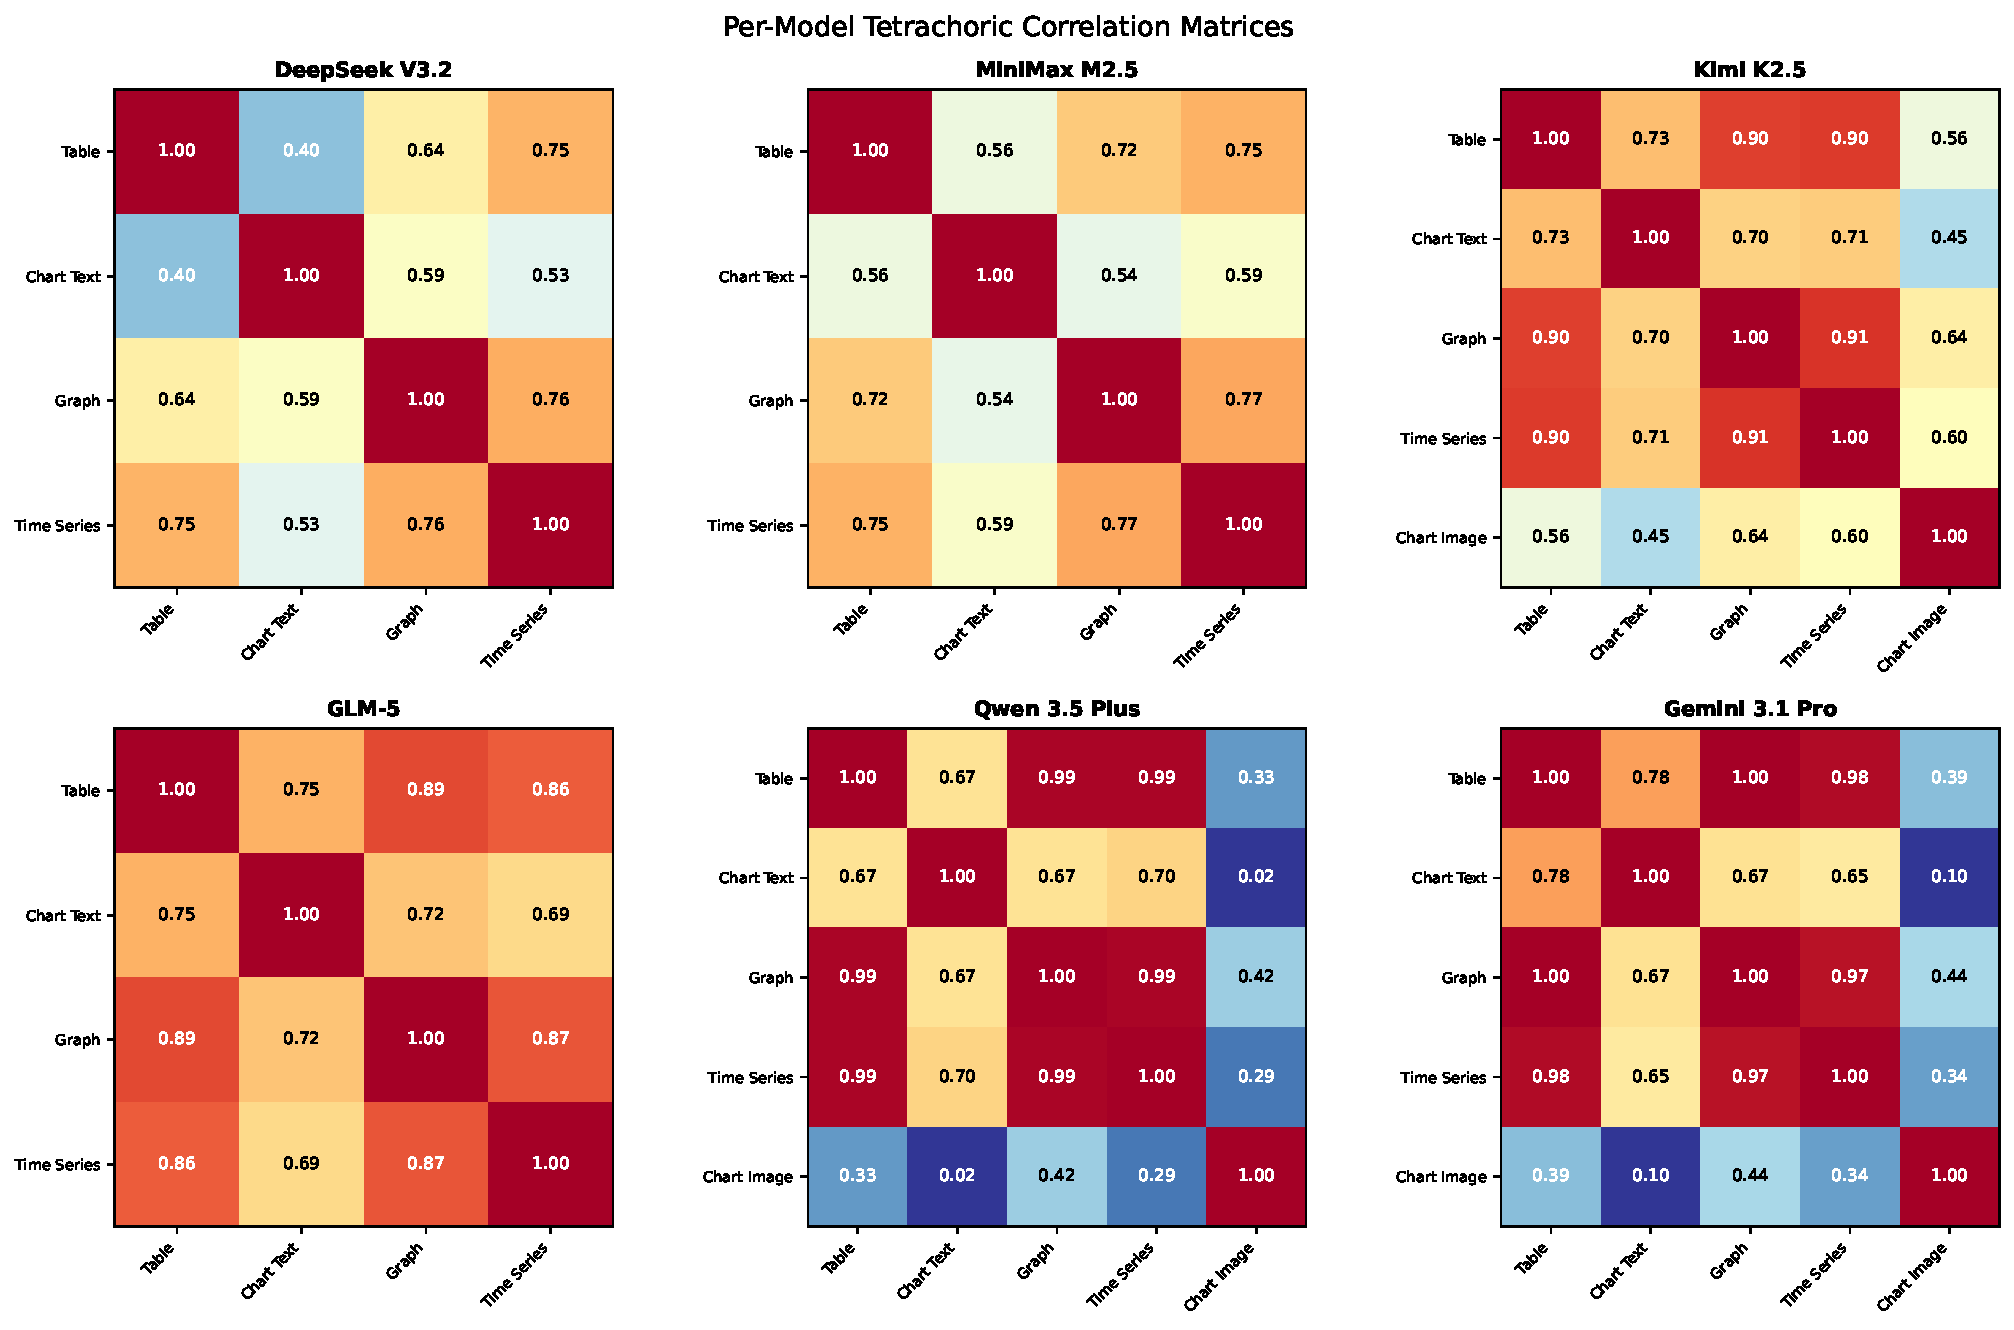
\includegraphics[width=\textwidth]{fig6_per_model_heatmaps.pdf}
    \caption{Per-model tetrachoric correlation matrices across all evaluated formats.}
    \label{fig:permodel}
\end{figure*}

\section{Accuracy by Question Type and Format}
\label{app:qtype_format}

Table~\ref{tab:qtype_full} provides a complete breakdown of accuracy by question type for each model, averaged across text formats.

\begin{table*}[t]
\centering
\small
\begin{tabular}{lccccccc}
\toprule
\textbf{Model} & \textbf{Q1} & \textbf{Q2} & \textbf{Q3} & \textbf{Q4} & \textbf{Q5} & \textbf{Q6} & \textbf{Q7} \\
\midrule
DeepSeek V3.2 & 98.2 & 96.7 & 94.0 & 99.9 & 95.5 & 98.3 & 81.6 \\
MiniMax M2.5 & 98.1 & 95.5 & 93.7 & 100.0 & 91.3 & 98.2 & 78.2 \\
Kimi K2.5 & 82.7 & 89.4 & 70.7 & 92.4 & 86.0 & 80.4 & 29.7 \\
GLM-5 & 97.8 & 95.6 & 78.3 & 99.6 & 94.1 & 97.7 & 46.6 \\
Qwen 3.5 Plus & 87.5 & 93.5 & 87.8 & 96.2 & 89.3 & 86.6 & 84.3 \\
Gemini 3.1 Pro & 90.6 & 95.2 & 90.5 & 97.4 & 91.4 & 88.8 & 87.8 \\
\bottomrule
\end{tabular}
\caption{Accuracy (\%) by question type across all models (averaged across text formats).}
\label{tab:qtype_full}
\end{table*}

\end{document}
